% Q1 classification section

\subsection{Problem Formulation}
We study binary sentiment classification on movie reviews. Given a review $x$, the task is to predict a label $y \in \{0,1\}$ where $0$ denotes negative sentiment and $1$ denotes positive sentiment. The goal is to compare sparse, dense, and contextual representations under a consistent evaluation protocol.

\subsection{Dataset Description}
We use the IMDb dataset with the official train and test splits, and create a stratified 10\% validation split from the training set (seed 42). The data are balanced across classes.

\begin{table}[H]
\centering
\caption{IMDb dataset statistics.}
\begin{tabular}{lrrrr}
\toprule
\textbf{Split} & \textbf{Examples} & \textbf{Avg Len} & \textbf{Positive} & \textbf{Negative} \\
\midrule
Train & 22,500 & 233.86 & 11,250 & 11,250 \\
Validation & 2,500 & 233.17 & 1,250 & 1,250 \\
Test & 25,000 & 228.53 & 12,500 & 12,500 \\
\bottomrule
\end{tabular}
\end{table}

\subsection{Methodology}
\textbf{Preprocessing and tokenization.} We compare two tokenization strategies: (i) a classical pipeline using NLTK word tokenization with optional lowercasing and stopword removal, and (ii) the DistilBERT tokenizer for contextual modeling. For the classical pipeline, we run an ablation over four configurations (A1--A4) and pick the best validation accuracy. A truncation study shows that larger token budgets improve validation accuracy (100 tokens: 0.8444, 200 tokens: 0.8720, 400 tokens: 0.8948).

\textbf{Models.}
\begin{itemize}[leftmargin=*]
		\item \textbf{TF-IDF + Logistic Regression} (sparse): unigram and bigram TF-IDF features with linear classifier.
		\item \textbf{BiLSTM + GloVe} (dense static): word embeddings initialized with GloVe 100d, BiLSTM encoder, mean pooling, and linear output.
		\item \textbf{DistilBERT} (contextual): fine-tuned DistilBERT for sequence classification.
\end{itemize}

\subsection{Experimental Setup}
We use fixed seed 42, a stratified validation split, and evaluate once on the test set. Metrics are Accuracy and Macro-F1. Training time is recorded for each model. Confusion matrices and training curves are saved for analysis.

\subsection{Results}
\begin{table}[H]
\centering
\caption{Test set results for Q1.}
\begin{tabular}{lccc}
\toprule
\textbf{Model} & \textbf{Representation} & \textbf{Accuracy} & \textbf{Macro-F1} \\
\midrule
TF-IDF + LR & Sparse & 0.8966 & 0.8966 \\
BiLSTM + GloVe & Dense (static) & 0.8898 & 0.8898 \\
DistilBERT & Contextual & 0.9296 & 0.9296 \\
\bottomrule
\end{tabular}
\end{table}

\begin{figure}[H]
\centering
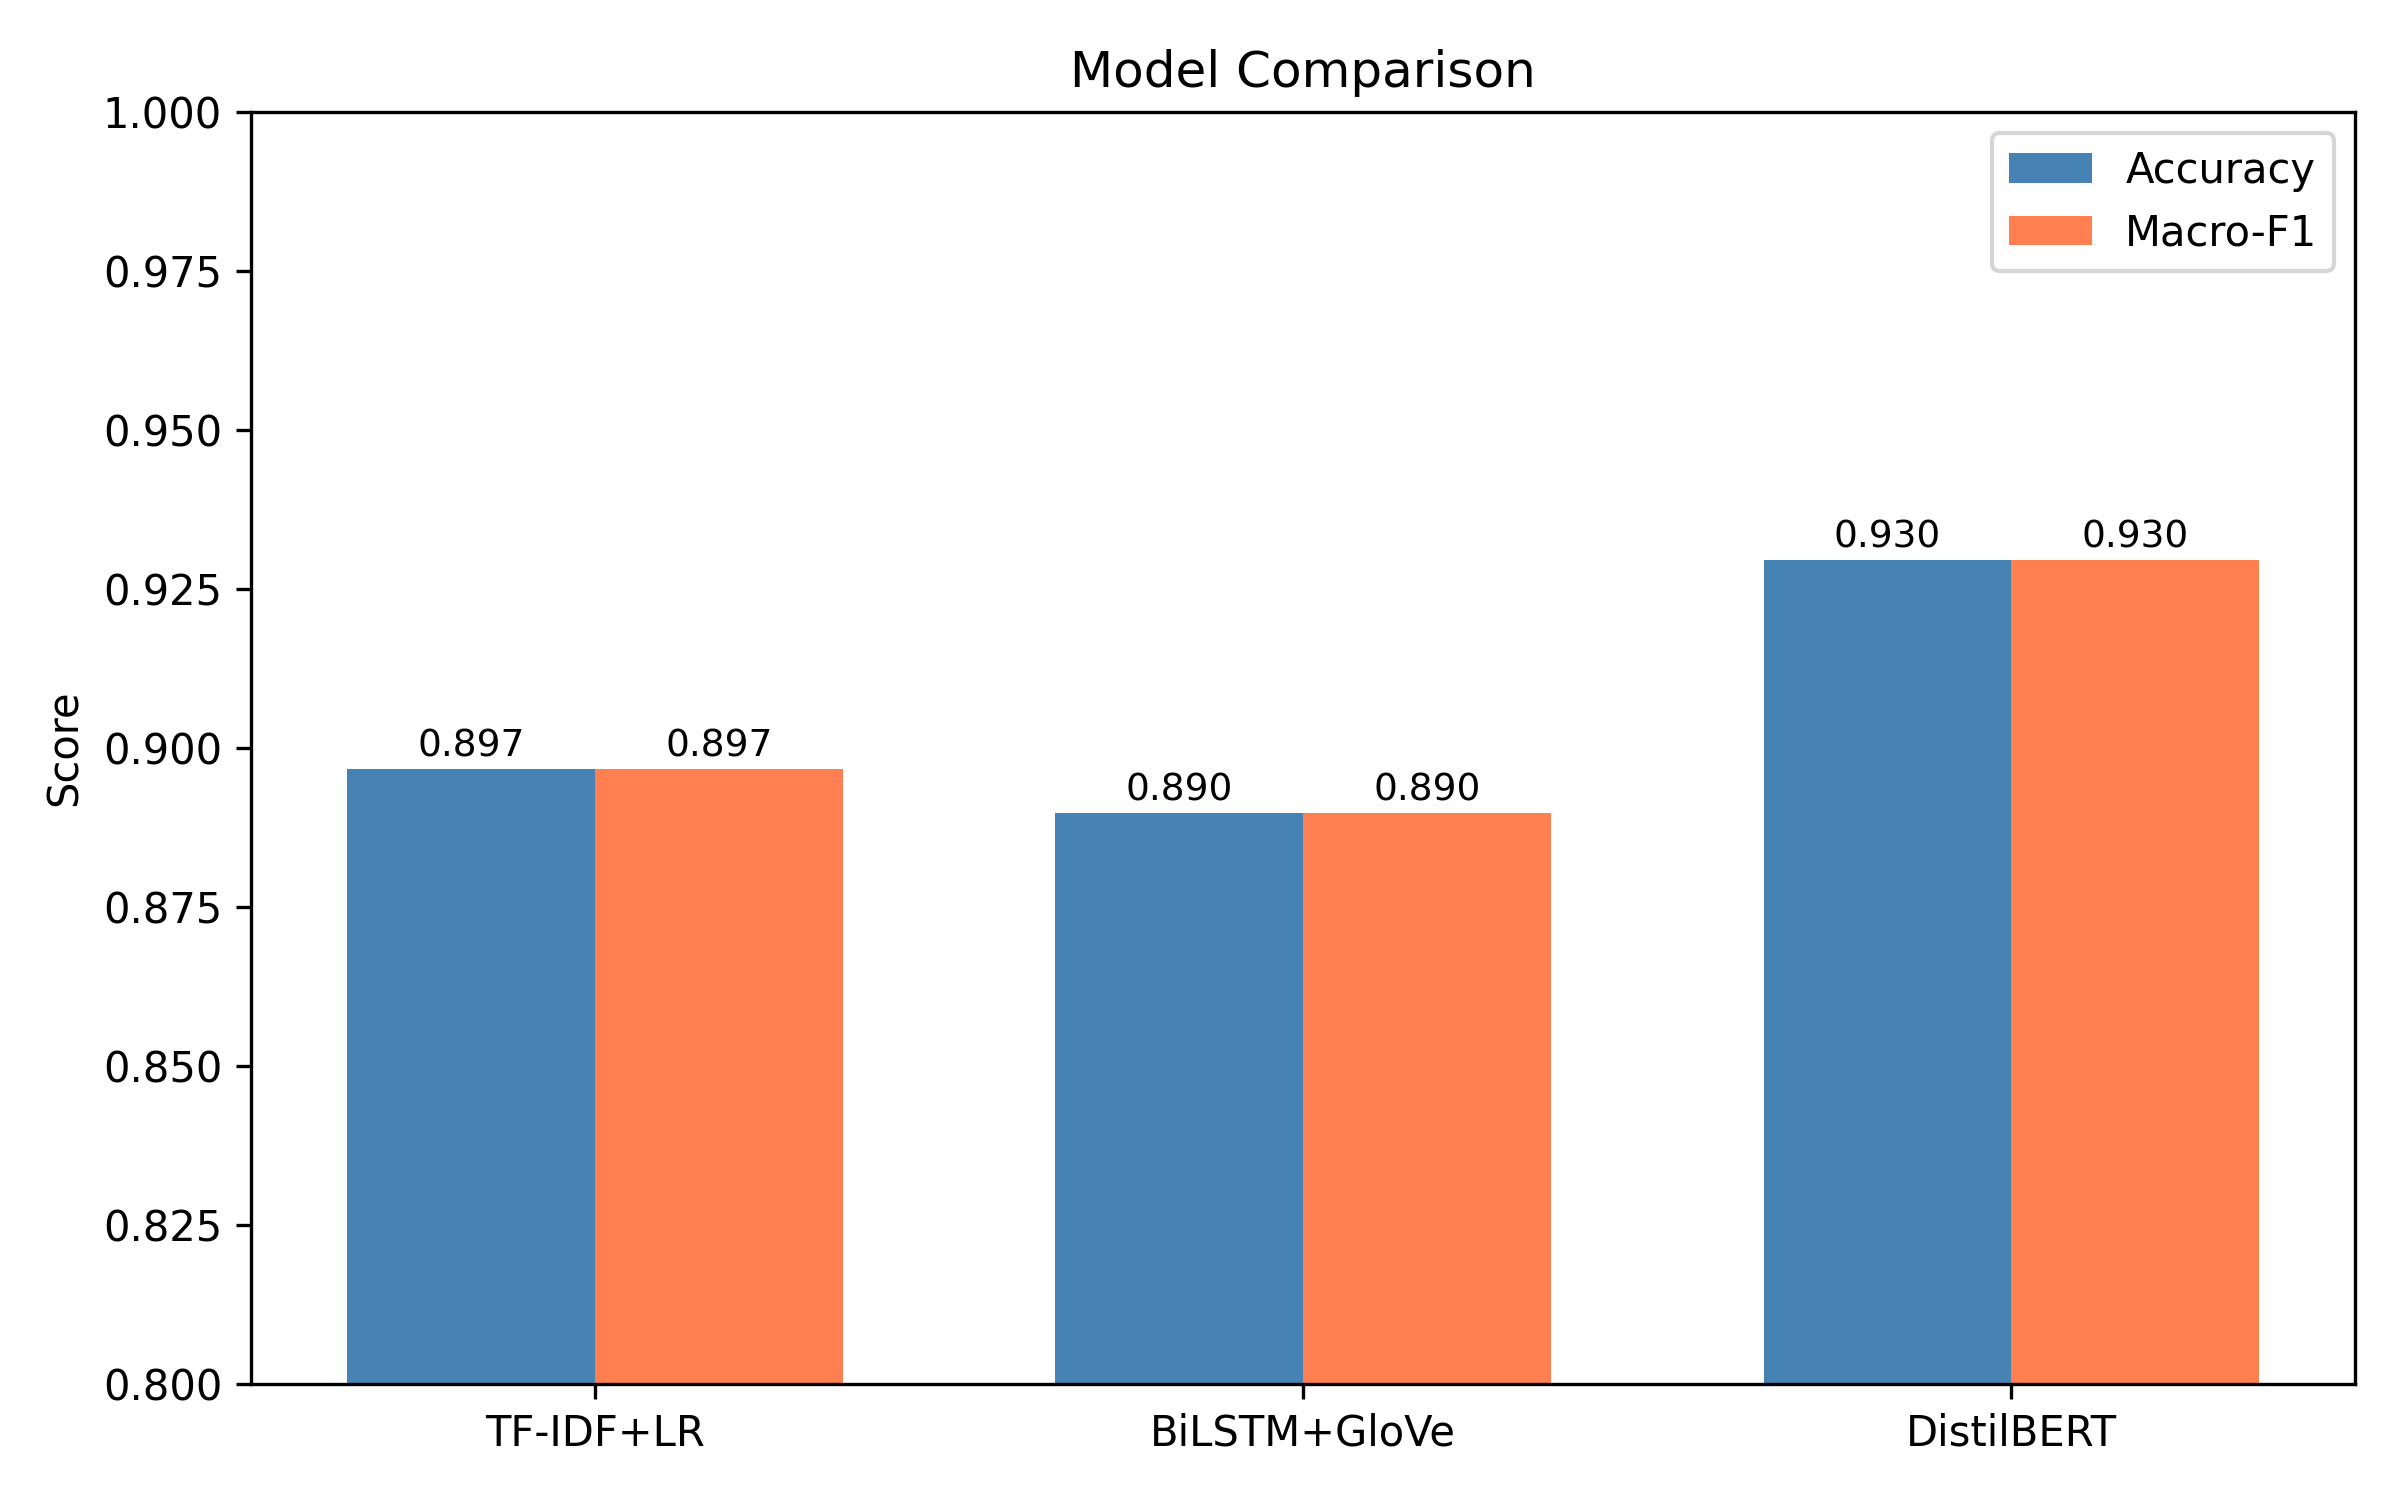
\includegraphics[width=0.78\linewidth]{../q1_classification/outputs/figures/model_comparison.png}
\caption{Accuracy and Macro-F1 comparison across models.}
\end{figure}

\begin{figure}[H]
\centering
\begin{subfigure}{0.32\linewidth}
	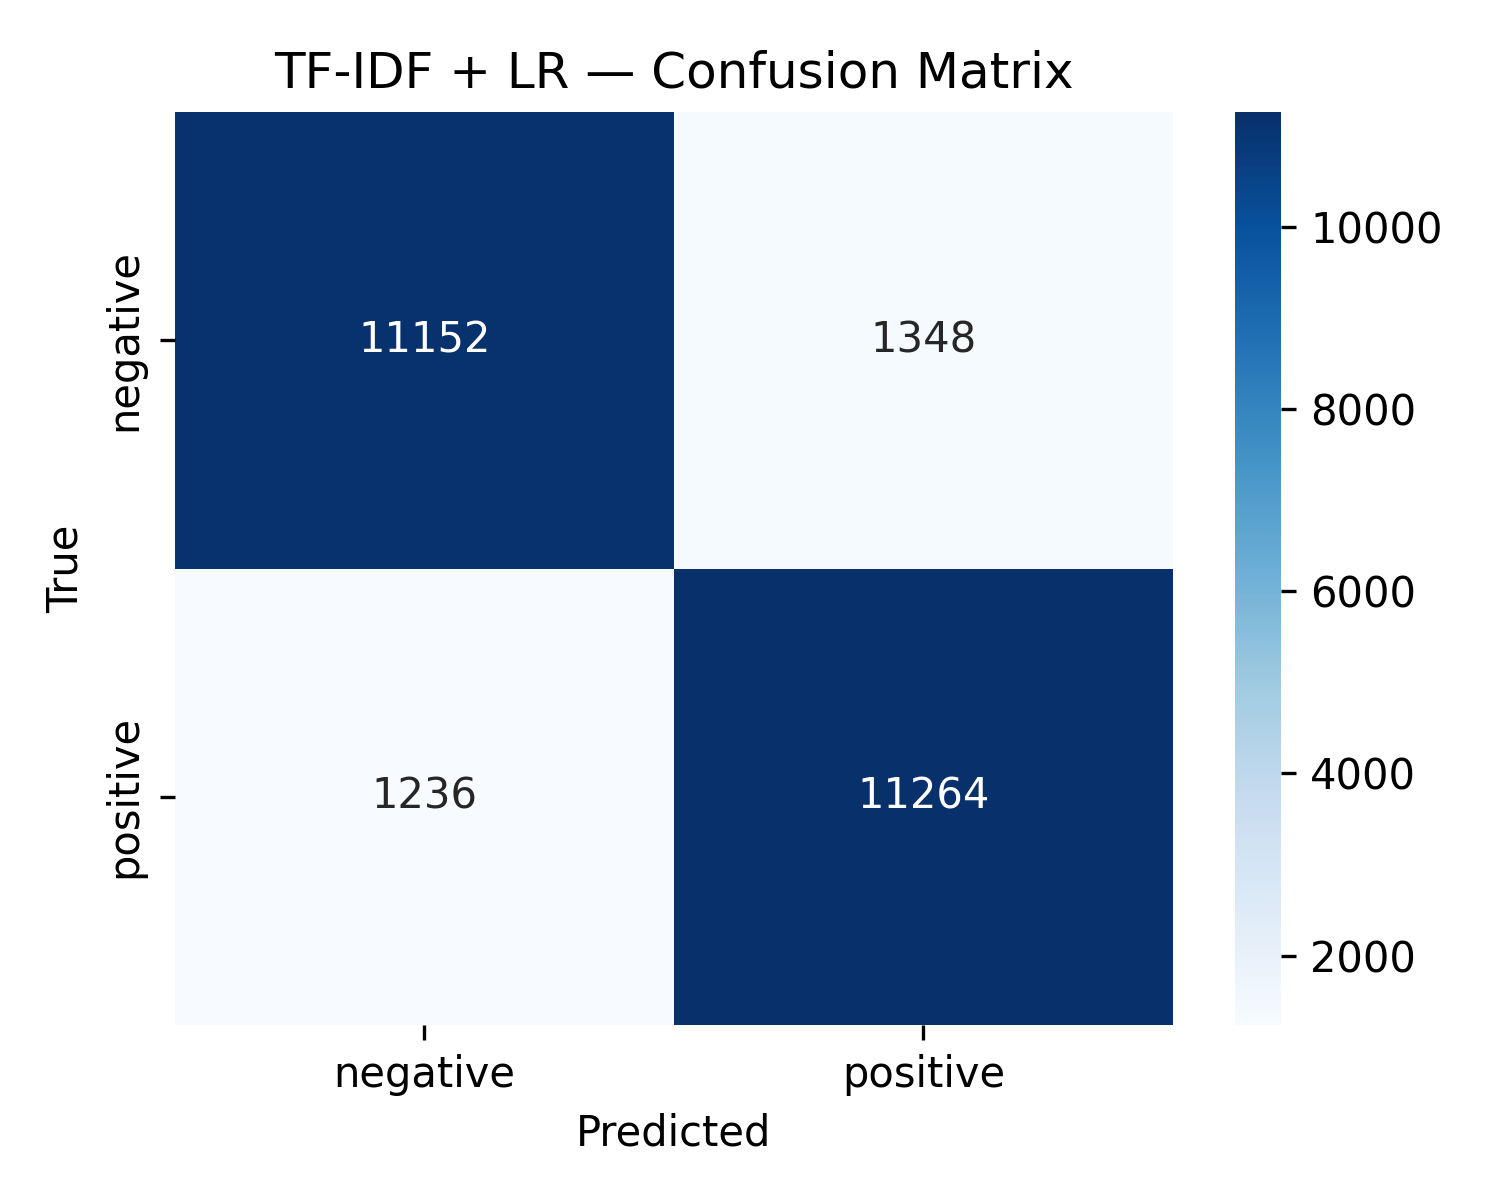
\includegraphics[width=\linewidth]{../q1_classification/outputs/figures/cm_tfidf.png}
	\caption{TF-IDF + LR}
\end{subfigure}
\begin{subfigure}{0.32\linewidth}
	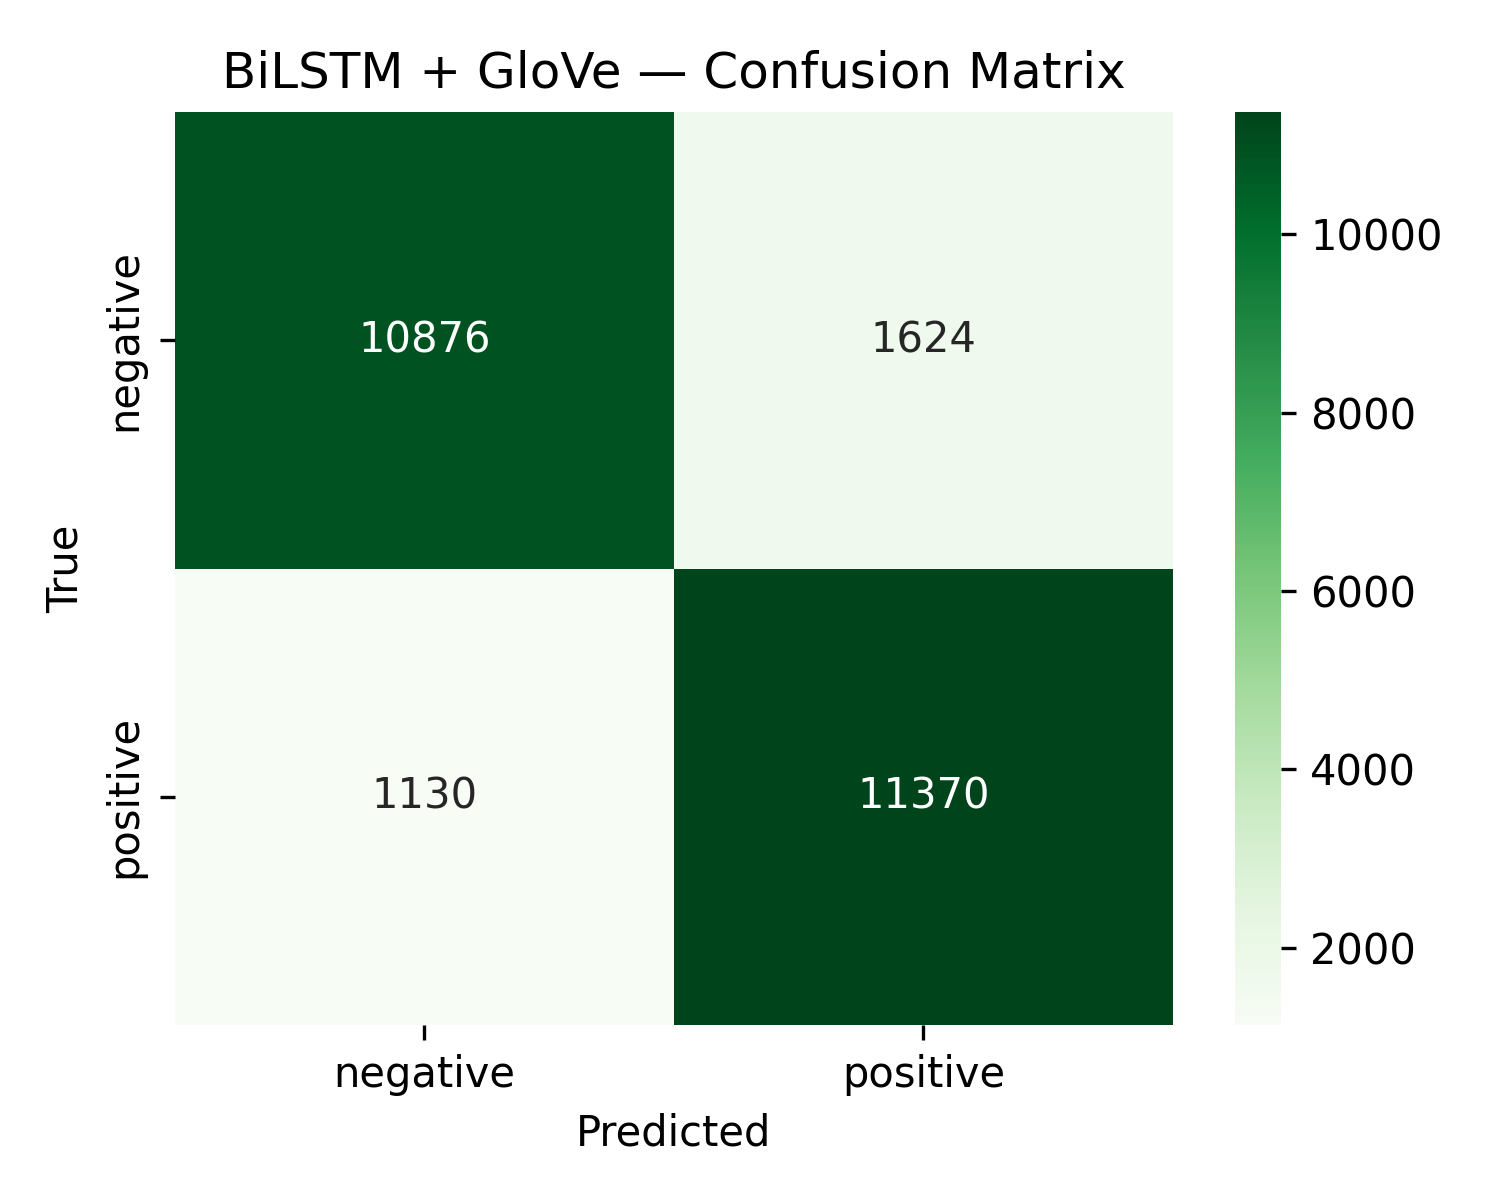
\includegraphics[width=\linewidth]{../q1_classification/outputs/figures/cm_bilstm.png}
	\caption{BiLSTM + GloVe}
\end{subfigure}
\begin{subfigure}{0.32\linewidth}
	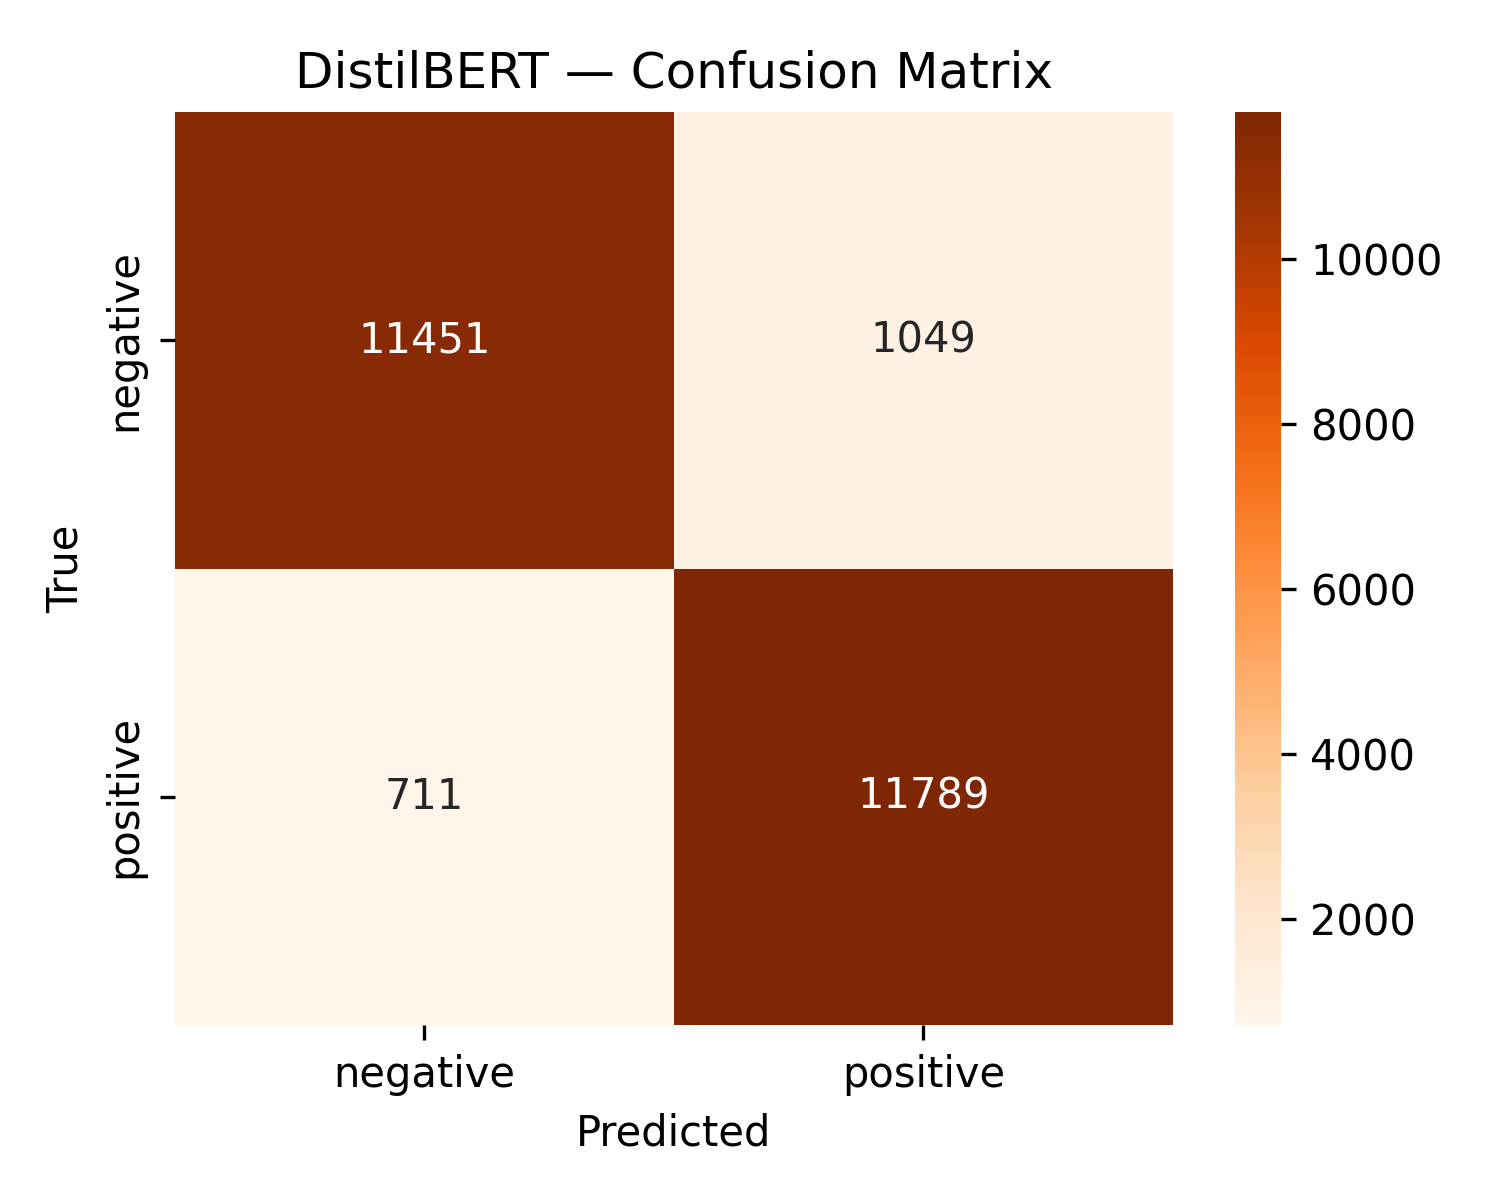
\includegraphics[width=\linewidth]{../q1_classification/outputs/figures/cm_distilbert.png}
	\caption{DistilBERT}
\end{subfigure}
\caption{Confusion matrices for all models.}
\end{figure}

\begin{figure}[H]
\centering
\begin{subfigure}{0.48\linewidth}
	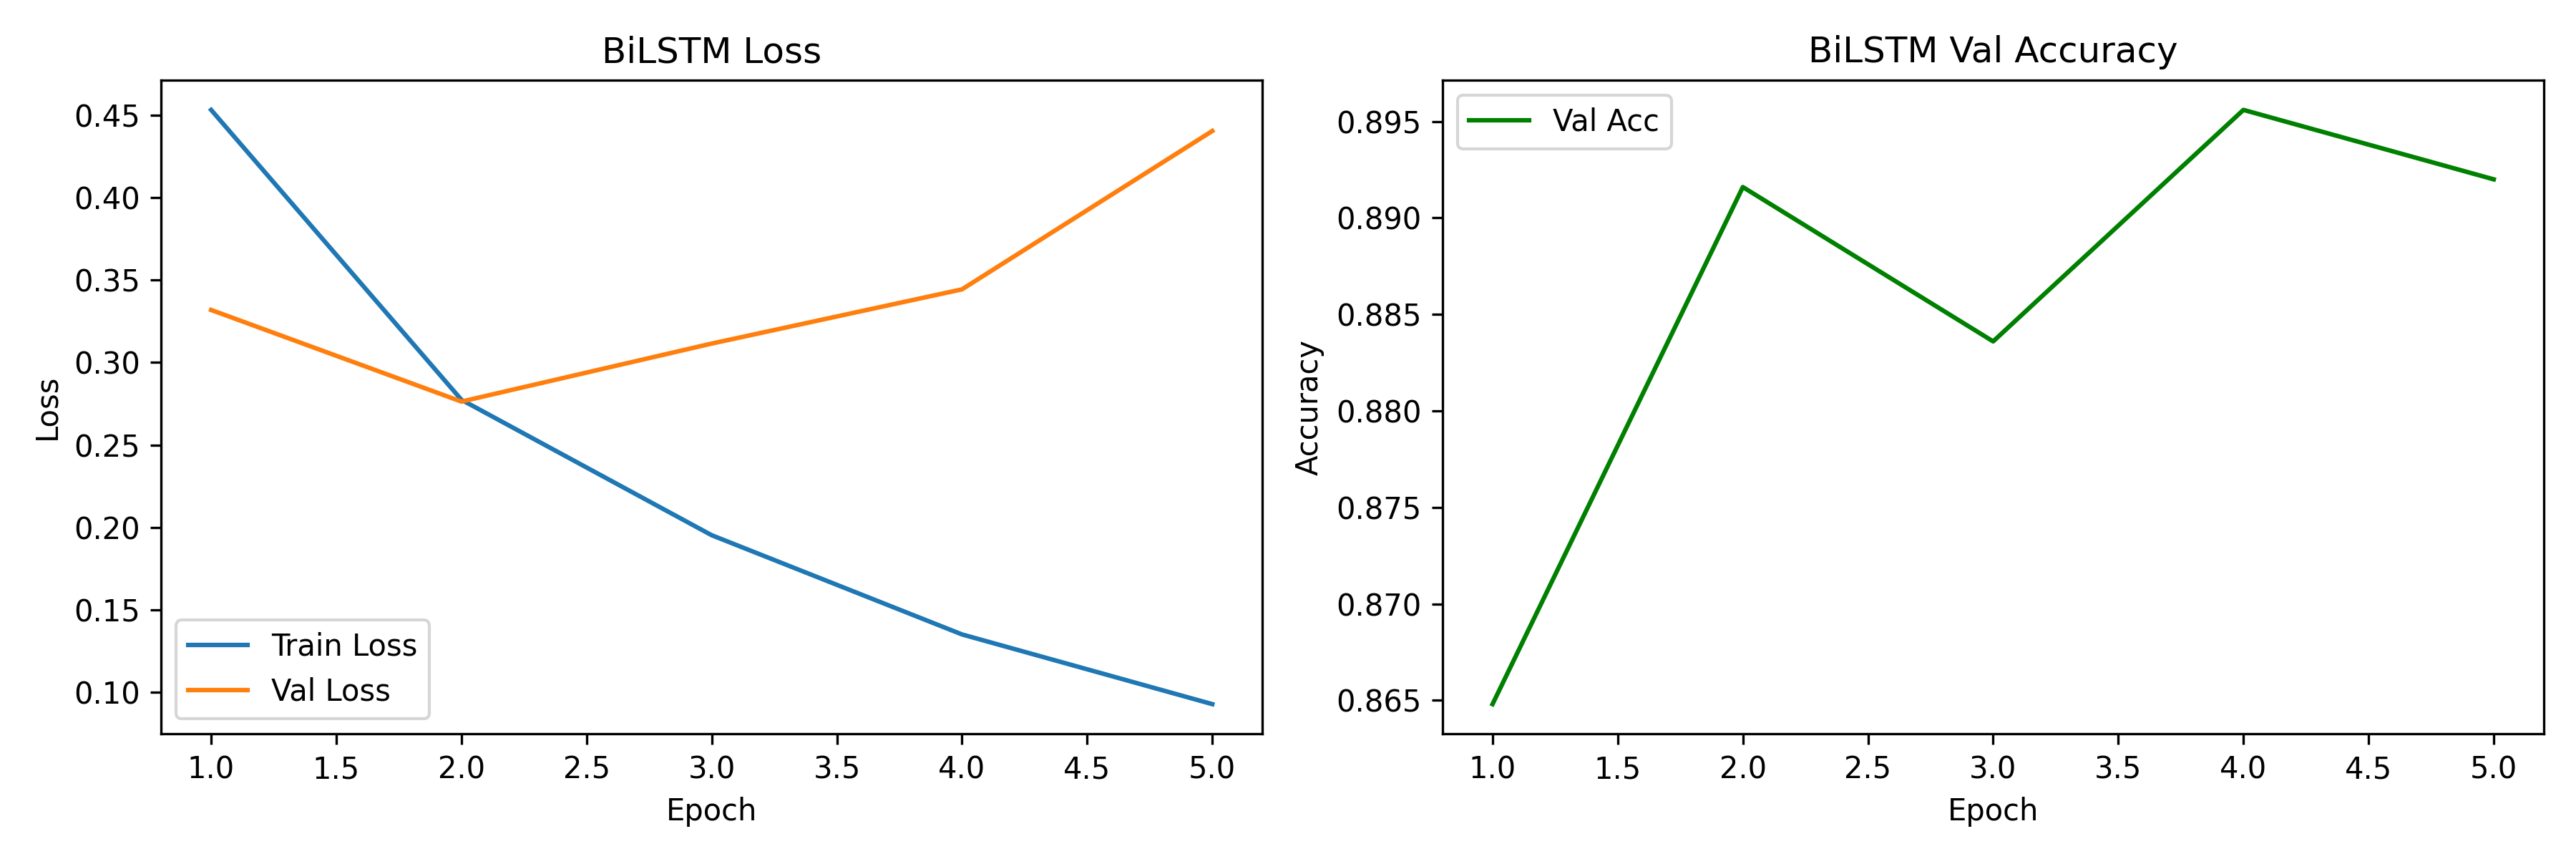
\includegraphics[width=\linewidth]{../q1_classification/outputs/figures/training_bilstm.png}
	\caption{BiLSTM training curves}
\end{subfigure}
\begin{subfigure}{0.48\linewidth}
	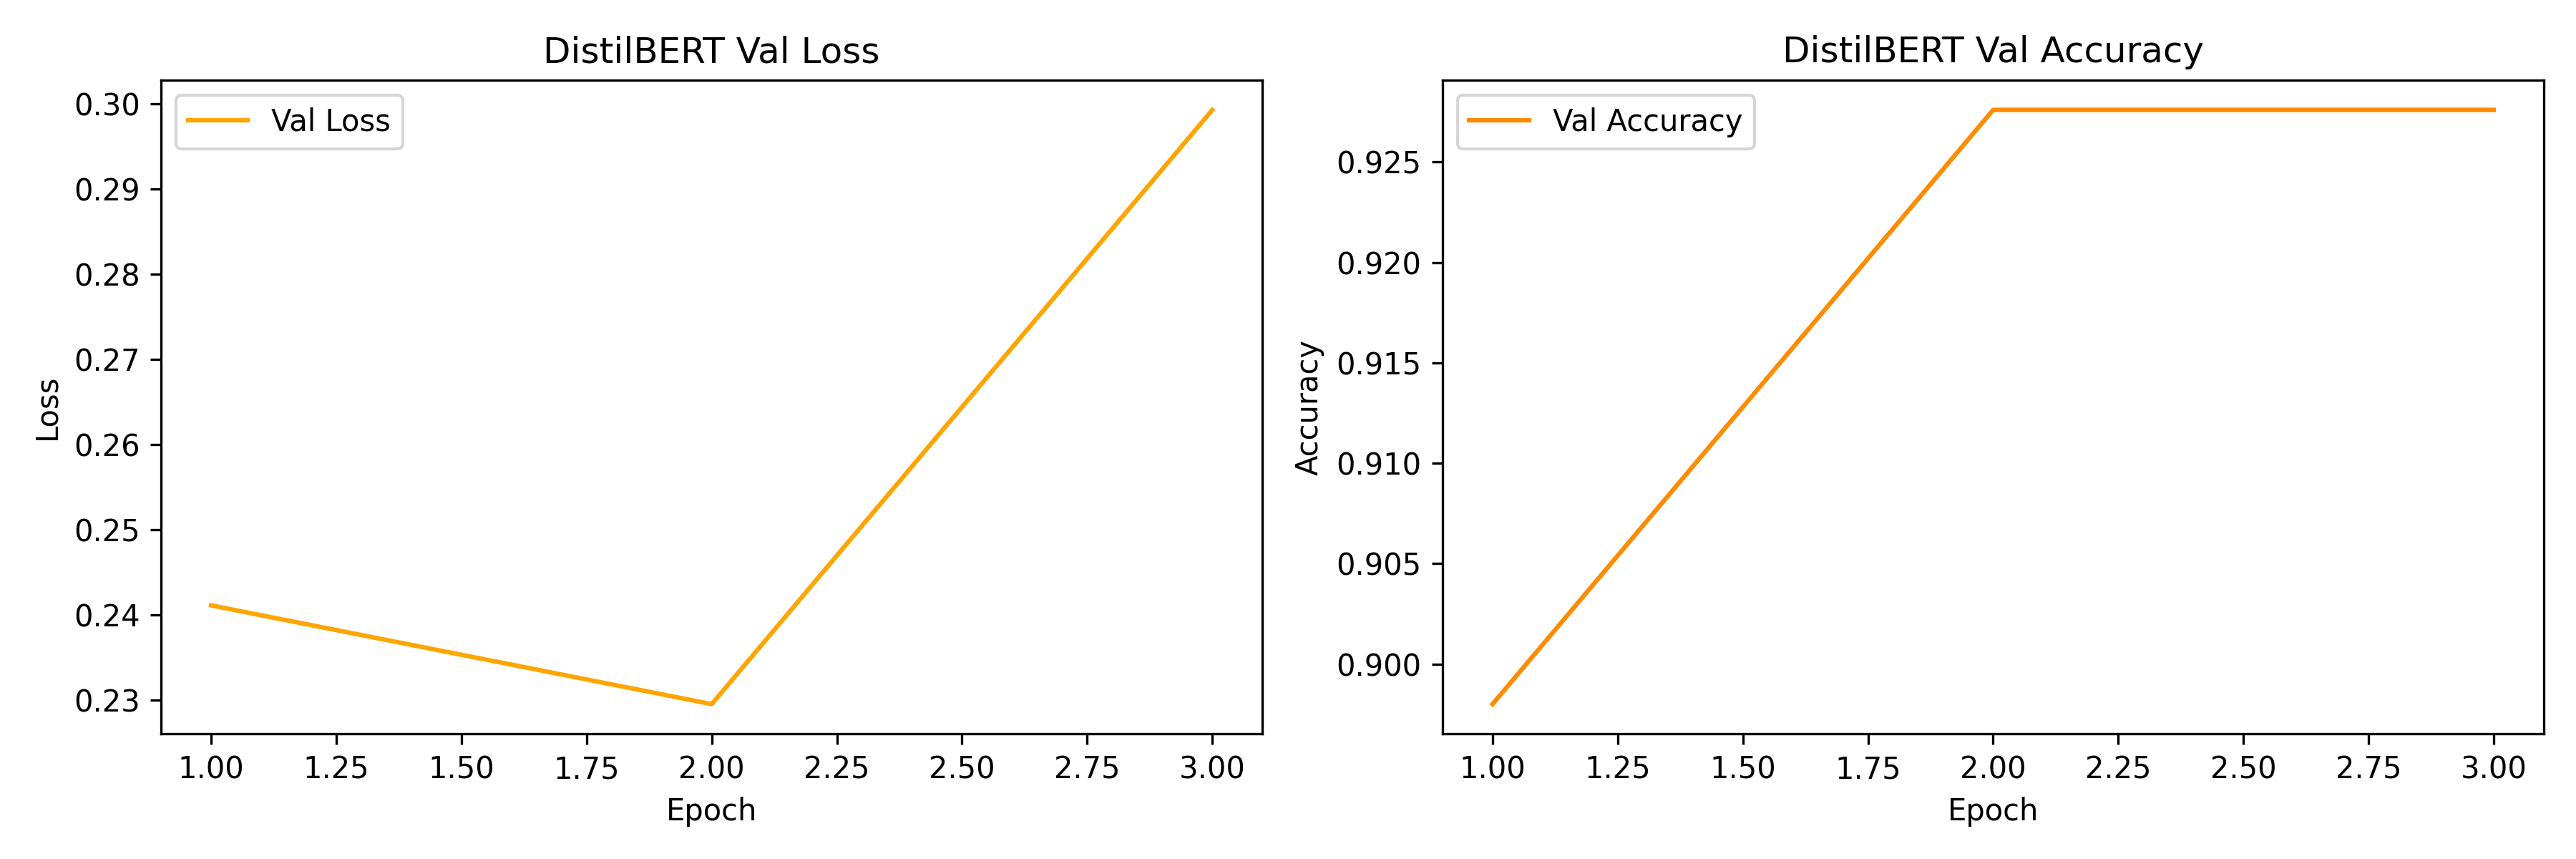
\includegraphics[width=\linewidth]{../q1_classification/outputs/figures/training_distilbert.png}
	\caption{DistilBERT training curves}
\end{subfigure}
\caption{Training dynamics for neural models.}
\end{figure}

\begin{figure}[H]
\centering
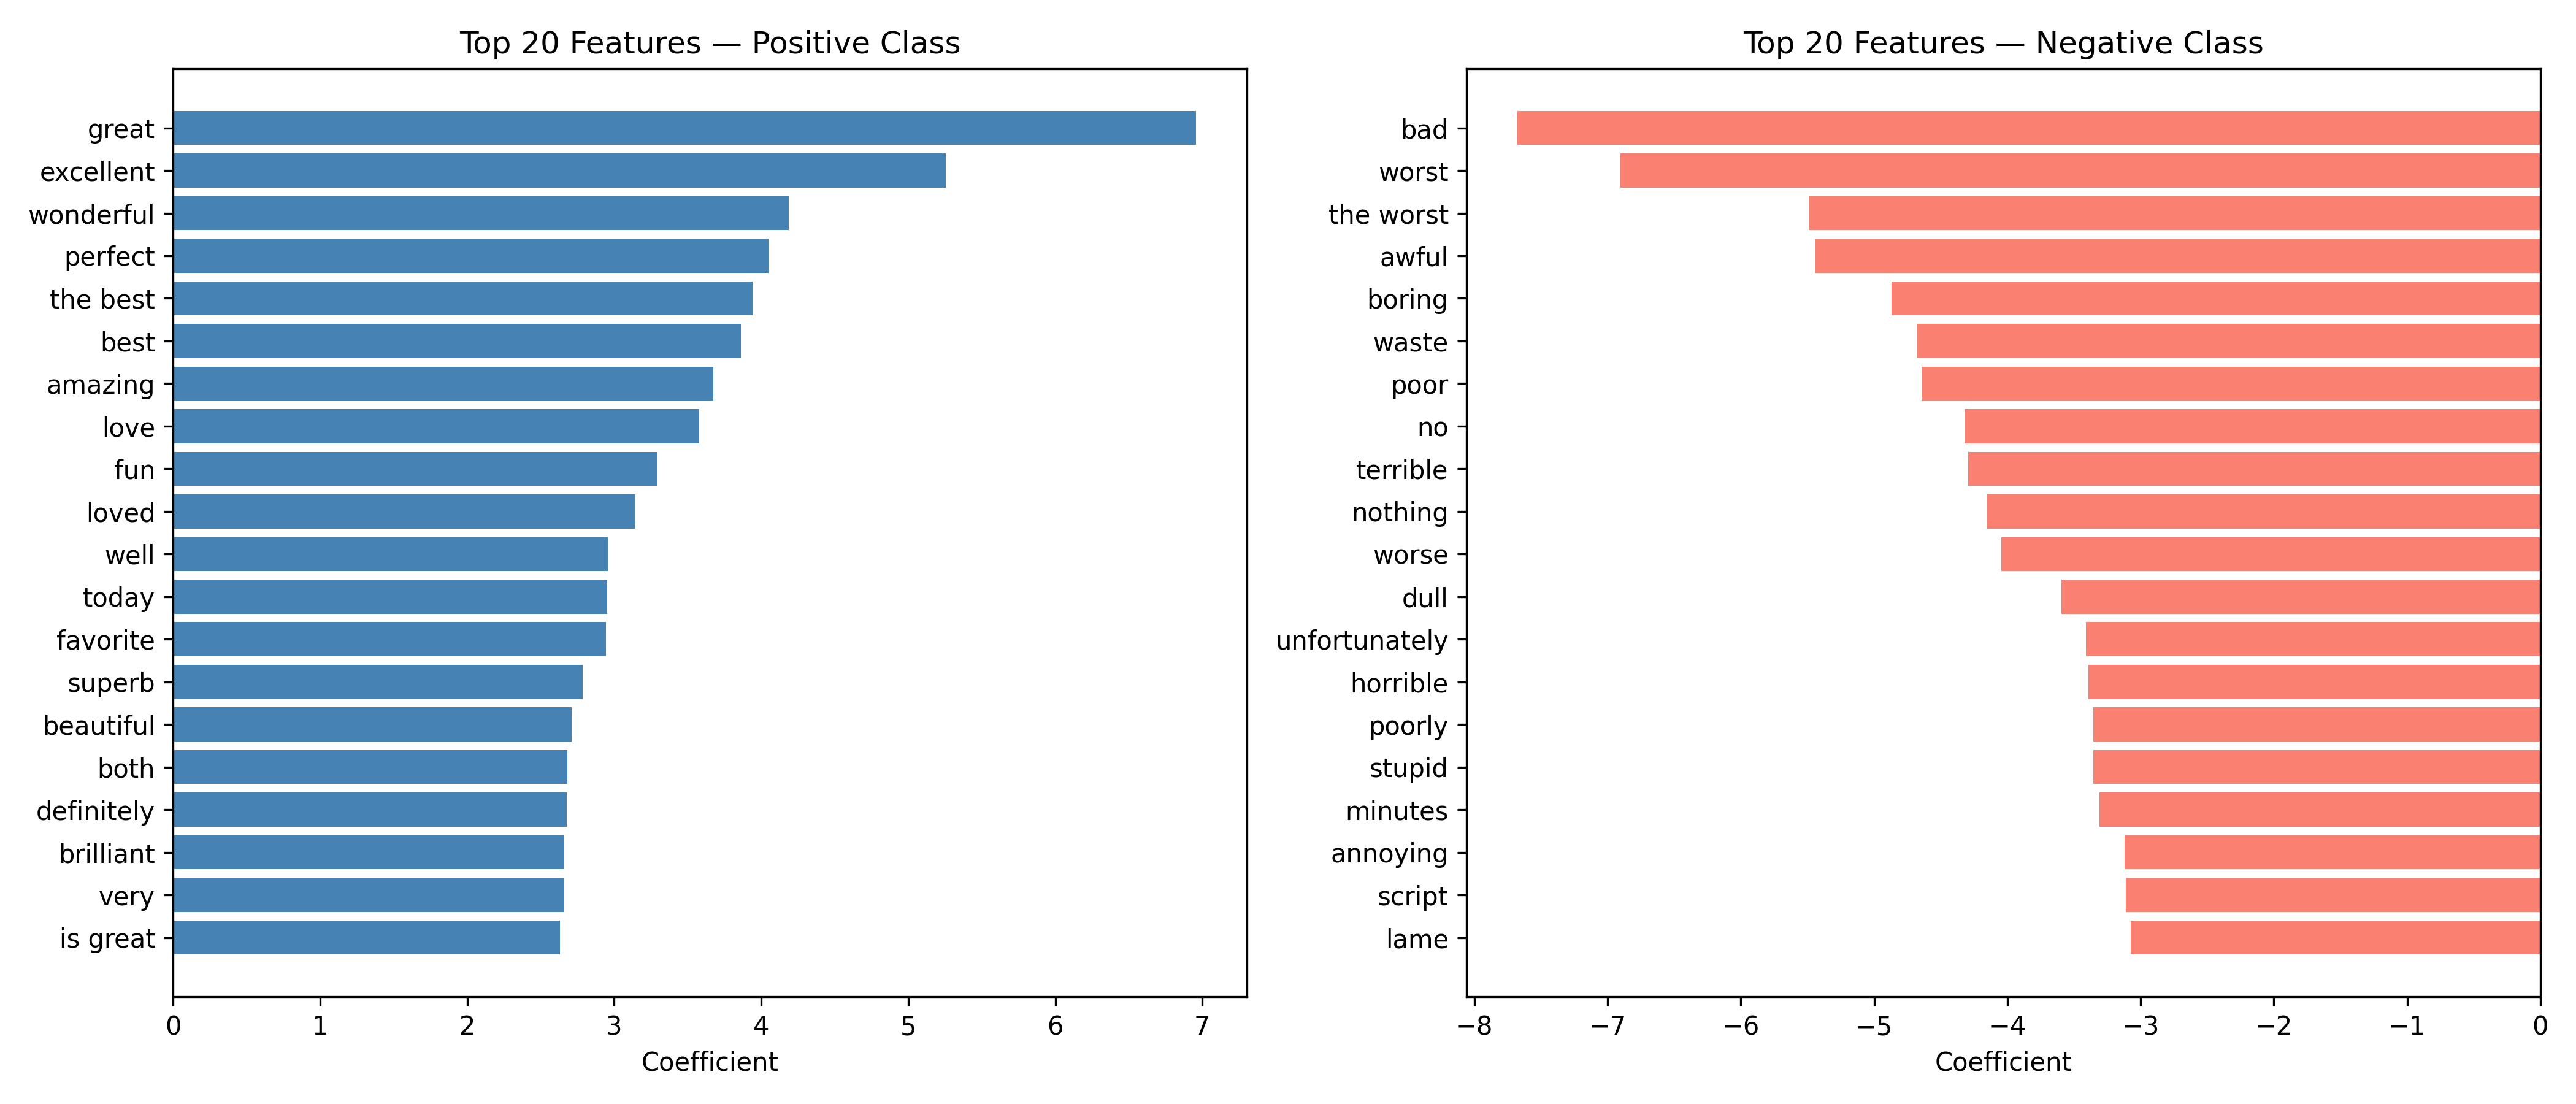
\includegraphics[width=0.9\linewidth]{../q1_classification/outputs/figures/tfidf_features.png}
\caption{Top TF-IDF features for positive and negative classes.}
\end{figure}

\subsection{Error Analysis}
We analyze misclassifications with a focus on common error patterns. The counts are: all three models wrong (774), TF-IDF only wrong (863), BiLSTM only wrong (875), DistilBERT only wrong (512). Five representative errors from the DistilBERT test set include:
\begin{itemize}[leftmargin=*]
		\item \textbf{Negation:} reviews with localized negation often flip sentiment cues (e.g., ``not like this movie").
		\item \textbf{Mixed sentiment:} positive and negative clauses co-occur, making the overall label ambiguous.
		\item \textbf{Domain terms:} film-specific words (e.g., ``plot'', ``acting'') can appear in both positive and negative contexts.
		\item \textbf{Sarcasm:} positive surface words mask negative intent.
		\item \textbf{Subtle tone:} mild criticism or praise without explicit sentiment markers.
\end{itemize}

\subsection{Discussion}
Sparse TF-IDF features are strong for sentiment cues and offer clear interpretability, but they struggle with long-range dependencies and nuanced phrasing. The BiLSTM benefits from sequence modeling but underperforms TF-IDF in this setup, likely due to limited capacity and the difficulty of long reviews. DistilBERT provides the best performance by leveraging contextual embeddings that capture semantics, negation, and long-distance dependencies more effectively, at the cost of higher training time and lower transparency.
